\documentclass[11pt,a4paper]{report}

\evensidemargin=0cm
\oddsidemargin=0cm
\topmargin=-1cm
\textheight=23.5cm
\leftmargin=0cm
\textwidth=18cm
\sloppy
\flushbottom
\parindent 1em
\hoffset -0.5in
\oddsidemargin  0pt
\evensidemargin 0pt
\marginparsep 10pt

\usepackage[utf8]{inputenc}
\usepackage[frenchb]{babel}
\usepackage[T1]{fontenc}

\usepackage{graphicx}

\usepackage{listings}
\usepackage{color}
\definecolor{lightgray}{rgb}{.9,.9,.9}
\definecolor{darkgray}{rgb}{.4,.4,.4}
\definecolor{purple}{rgb}{0.65, 0.12, 0.82}

\lstnewenvironment{OCaml}
                  {\lstset{
                      language=[Objective]Caml,
                      breaklines=true,
                      commentstyle=\color{purple},
                      stringstyle=\color{red},
                      identifierstyle=\ttfamily,
                      keywordstyle=\color{blue},
                      basicstyle=\footnotesize
                    }  
                  }
                  {}
\lstnewenvironment{C}
                  {\lstset{
                      language=C
                      breaklines=true,
                      commentstyle=\color{purple},
                      stringstyle=\color{red},
                      identifierstyle=\ttfamily,
                      keywordstyle=\color{blue},
                      basicstyle=\footnotesize
                    }  
                  }
                  {}

\title{Rapport de projet\\Débogueur Visuel pour OCaml}
\author{Mathieu Chailloux\\Vincent Botbol}
\date\today

\begin{document}
\maketitle

\chapter{Introduction}

Bien que le langage OCaml soit considéré comme un langage sûr de par la sécurité de son typage statique et fort, % trouver +
l'utilisateur n'est pas à l'abri de problèmes algorithmique ou ... . La distribution de base du langage inclut %todo
un débogueur, \emph{ocamldebug}, en ligne de commande. Cependant, son utilisation est parfois mal adaptée au besoin du programmeur.

Notre projet tente de répondre à ces problèmes en apportant au débogueur une interface graphique simple ainsi quelques
outils supplémentaires facilitant l'emploi du logiciel. Nous nous approchons d'outils similaires
tel que \emph{ddd} pour \emph{gdb}, l'interface graphique du célèbre débogueur pour le langage C. Notre logiciel se concentre
principalement sur l'aspect ergonomique d'un  bien qu'une grande partie de notre travail visa à améliorer certains
aspects du débogueur déjà présent.
% ^ tourner ça plus correctement

Pour expliciter les forces et les faiblesses d'\emph{ocamldebug}, nous détaillerons, dans une première partie:
l'utilisation de cet outil et son fonctionnement interne.

Nous présenterons ensuite notre outil, les extensions développées et certaines de ses possibilités d'améliorations.

\chapter{Ocamldebug}

\section{Présentation}

%topo
%exemple d'utilisation
%liste des commandes

\section{\'Evénements de débogage}
\section{Communication avec la machine virtuelle}
\section{Limitations et inconvénients} % transition


\chapter{OCabug}

%intro : ce qu'on a fait
%présentation des différentes extensions, installation, ocaml 3.12...
%patch du compilo


\section{Présentation de l'interface}

L'interface graphique de l'application a entièrement été réalisée avec LablGtk, le ``binding'' de Gtk pour OCaml.
Elle assure un confort visuel à l'utilisateur en permettant un accès rapide aux commandes les plus utilisées ainsi
que l'observation directe des différents fichiers sources permettant de constater la position courante 
et des différents ``breakpoints'' du programme. Le toplevel d'ocamldebug est également présent pour afficher
les différentes actions du débogueur et les sorties textuelles engendrées.

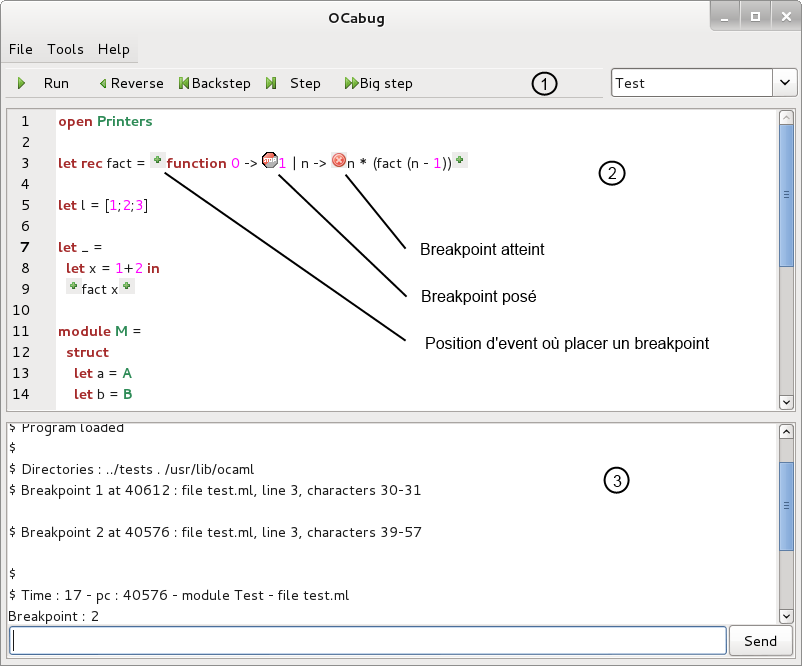
\includegraphics{screen_exec}

\begin{enumerate}
\item Barre d'outils et séléction du module à afficher
\item Affichage du fichier source du module courrant enrichi des événements de débogage activables
\item Informations textuelles et invite de commande
\end{enumerate}

L'utilisateur a activé deux ``breakpoints'' en cliquant sur les ``+'' présent dans l'affichage du source.
Il démarre ensuite le programme en appuyant sur \emph{Run} qui s'arrête au premier breakpoint rencontré,
changeant temporairement son icône ``Stop'' par un ``X'' rouge.

\subsection{Barre d'outils}

Les différents boutons incluent dans la barre d'outils réunissent les commandes les plus communes lors de l'utilisation:
\begin{itemize}
\item Run -- Permet de lancer le programme. Celui-ci s'arrêtera lorsqu'un breakpoint sera rencontré ou simplement à la fin du programme.
\item Reverse -- Action symétrique au Run; Parcours le programme en sens inverse toujours en s'arrêtant au breakpoint ou au début du programme.
\item Backstep -- Recule d'un événement de débogage.
\item Step -- Avance d'un événement de débogage
\item Big step -- Avance au prochain événement en omettant ceux de module différent.
\item Liste des modules -- Permet de basculer l'affichage des différents fichiers sources présents.
\end{itemize}

\subsection{Code source}

Le panneau du code source a d'autres emplois que la simple visualisation du programme. 
Il permet également à l'utilisateur de poser des breakpoints dans le code au niveau des événements du débogage.

Chaque icône a sa signification particulière:
\begin{itemize}
\item Symbole ``+'' vert -- \'Evénement de débogage: un click active la pose d'un breakpoint à cet endroit du code
\item Symbole ``+'' gris entouré -- Position actuelle du programme
\item Panneau ``Stop'' -- Breakpoint actif: un click le retire
\item Croix rouge -- Position actuelle du programme ayant atteint un breakpoint
\end{itemize}

\subsection{Toplevel}

La console affichant le toplevel permet à l'utilisateur de constater les différents affichages du programme
et du débugueur. Les commandes entrées par l'utilisateur dans la zone de saise sont interprétées de la même
manière que pour ``ocamldebug'' en supportant également nos propres commandes.

\section{Placement par rapport à Ocamldebug}

Notre implémentation se base sur le noyau d'``ocamldebug''. Nous avons repris le code originel et
avons adapter les mécanismes d'entrées/sorties console pour les convertir à une utilisation
graphique. Il nous a ensuite fallu lié les différents composants de l'interface aux fonctions du débogueur
tout en maintenant une cohérence entre les commandes entrées manuellement et l'utilisation de l'interface.
Nous maintenons ainsi toutes les fonctionnalités originelles du débogueur. 

La modification du noyau est restée nécessaire pour pouvoir nous permettre d'ajouter nos propres commandes.
...

%nécessite le compilo + lablgtk (ici?)
\section{Implémentation des extensions}

Nous avons principalement deux extensions à notre disposition.
Premièrement, la commande ``Big step''. A plusieurs moments, le programmeur ne
peut ne pas souhaiter se déplacer dans des modules externes lors d'un débogage.
Notre commande considère alors le module courant et passe au prochain événement
qu'il rencontrera dans ce même module.

Techniquement, cette commande agit de la même manière qu'un ``step'' en vérifiant 
en plus, à chaque avancement, que l'événement appartient bien au même module. 
Si ça n'est pas le cas, on continue jusqu'à ce que la condition soit satisfaite.

Nous disposons également d'une instruction de déplacement filtrant les modules
appartenant à la librairie standard. En effet, la plupart du temps, nous ne souhaitons
pas rentrer dans le code de la bibliothèque standard. Nous pouvons ainsi nous abstraire
des différentes fonctions que l'utilisateur considère comme sûres pour nous consacrer
exclusivement au code en cours de débogage. On peut noter aussi la présence d'une option
pour ajouter ou enlever des modules à la liste des filtres actifs. 

Pour implémenter un tel comportement, nous récupérons tout d'abord la liste des modules standards
d'OCaml grâce à la variable d'environnement contenant le chemin vers leur dossier. Nous pouvons ensuite
filtrer selon le module de l'événement atteint si celui-ci est éligible ou non.
% + ?

Ce comportement concerne le bouton ``step'' de l'interface et est activé par défaut. 
Ceci peut, à tout moment, être modifié via le menu de l'application.

\section{Améliorations possibles}
%threads
%compteur

\chapter{Conclusion}

%whine sur le bordel que c'était
%compréhension du débogueur
%adaptation d'ocamldebug

\chapter{Annexes}

\section{Exemples}
\section{Liste des commandes}

\end{document}
